\documentclass[preprint,12pt]{elsarticle}

\usepackage[T1]{fontenc}
\usepackage[utf8]{inputenc}
\usepackage{amsmath,amssymb,amsthm}
\usepackage{booktabs}
\usepackage{graphicx}
\usepackage[hidelinks]{hyperref}

\journal{Computers \& Industrial Engineering}

\newtheorem{lemma}{Lemma}
\newtheorem{proposition}{Proposition}

\begin{document}

\begin{frontmatter}

\title{Inventory age and store minimum remaining shelf life in warehouse-to-store distribution}

\author{Author Name}
\address{Affiliation}

\begin{abstract}
Retail cold-chain warehouses hold batches of different ages, and stores often reject deliveries whose remaining shelf life is below a store-specific minimum (MLOR). Because travel time consumes shelf life, the age of the inventory at a warehouse determines which stores that warehouse can serve. We study a single-period, deterministic, single-echelon, unit-demand location-routing problem in which opening warehouses, assigning stores, routing vehicles, and selecting the inventory age are decided together. The problem is formulated as a mixed-integer program; the shelf-life condition reduces to an arrival deadline that depends on the serving warehouse's age and the store's threshold. We solve small and medium instances exactly by subset dynamic programming and develop an age-feasible adaptive large neighbourhood search (ALNS) for larger instances. On 8- and 12-store synthetic instances, an age-aware plan is never worse than an age-blind plan and is better in 9/10 and 7/10 cases. With a destroy size selected on a development set, the ALNS reaches the exact optimum in 9/10 held-out twelve-store instances (mean gap 1.78); the default setting reaches 8/10 (mean gap 13.43). At 20 stores it improves a greedy plan by 1301.1 on average. Three practical policies are worse on average than the exact and ALNS solutions, and a $2\times 2$ check shows that the age--distance--threshold interaction, rather than the cold-chain label, drives the difference. All parameters are synthetic; the results are conditional and do not constitute field estimates.
\end{abstract}

\begin{keyword}
inventory age \sep shelf life \sep location-routing \sep adaptive large neighbourhood search \sep cold chain
\end{keyword}

\end{frontmatter}

\section*{Highlights}
\begin{itemize}
\item Inventory age and store MLOR create an age--distance--threshold matching problem.
\item Age-aware plans can open different warehouses and assign stores differently.
\item Exact subset DP solves 8- and 12-store instances; ALNS is near-optimal at 12.
\item A freshest-first rule is a reasonable default; oldest-first is not.
\item Gains are conditional on rejection cost and unit-demand scope.
\end{itemize}

\section{Introduction}

A cold-chain distribution network moves fresh products from warehouses to retail stores. We model the warehouse-to-store stage; the upstream central-warehouse-to-regional-warehouse stage is outside the model. The inventory at a warehouse is not homogeneous: batches differ in production date and therefore in remaining shelf life. Stores commonly impose a minimum remaining shelf life at delivery, either as a contractual acceptance rule or as a markdown trigger. A delivery that arrives after a long route may be rejected even when the vehicle arrives within its time window, because the product has spent too much of its shelf life in transit.

The operational consequence is that travel time acts as a shelf-life tax. If a batch of age $a$ leaves warehouse $i$ and reaches store $j$ after time $t$, the remaining shelf life is $L-a-t$, and it must be at least the store's threshold $m_j$. An old batch therefore has a shorter effective service radius: it can serve nearby stores, or stores with a low threshold, but not distant stores with a high threshold. This relation couples decisions that are often studied separately: which warehouses to open, which store is assigned to which warehouse, in what order a vehicle visits its stores, and which inventory age is used.

We study this coupling in a single-period, deterministic setting. The question is not whether shelf life matters---it obviously does---but whether the age--distance--threshold relation changes the network design in a way that a planner who ignores age would miss. We formulate the problem as a mixed-integer program, solve small and medium instances exactly by subset dynamic programming, and develop an age-feasible ALNS for larger instances. The experiments compare age-aware and age-blind plans, three practical assignment policies, and an exact lower bound at 20 stores.

The paper is positioned against three literatures. Perishable inventory-routing models track remaining shelf life and freshness but typically keep the depot fixed \citep{coelho2014,crama2018}. Two-echelon inventory-routing and location-routing models decide network structure and routes but do not model a store-specific delivery threshold \citep{govindan2014,rohmer2019}. The MLOR concept itself has been studied in an operations--marketing setting \citep{singh2022}, but not, to our knowledge, inside a location-routing model. The precise difference---warehouse age, store-specific threshold, and location-routing decided together---remains to be verified against the closest work, including \citet{qiu2019}, whose full text we could not obtain.

Three contributions follow. (i) Modeling: we formulate a location-routing model in which the shelf-life condition is an arrival deadline determined jointly by warehouse age and store threshold, and we state the operational assumptions that delimit its scope. (ii) Method: we give an exact subset dynamic program for small and medium instances and an age-feasible ALNS for larger ones; the ALNS neighborhood is chosen because cross-warehouse reassignment, not route reordering, is the move that the mechanism requires. (iii) Empirical: we compare against an age-blind exact plan, three practical policies and a rule-plus-local-search baseline, isolate the age--MLOR interaction with a $2\times2$ check, and report confidence intervals rather than only point estimates. We do not claim a new problem class; the evidence supports a conditional decision mechanism, not a field recommendation.

\section{Related work}

\subsection{Perishable inventory routing}

Perishable inventory-routing models combine replenishment, inventory and routing decisions when product quality decays over time. \citet{coelho2014} study joint replenishment, delivery and inventory policies for perishable products and show that age-dependent inventory materially changes the cost structure. \citet{crama2018} model a stochastic inventory-routing problem in which store inventory is disaggregated by remaining shelf life, issuing follows FIFO, and a stockout-probability service level is imposed; they report freshness and waste metrics in addition to profit. Their model is multi-period and keeps the depot fixed. Our setting is single-period and includes location decisions, and the threshold applies at delivery rather than as a stockout-probability service level.

\subsection{Two-echelon inventory routing and location-routing}

Two-echelon inventory-routing models decide how much to ship from a supplier to an intermediate depot and from the depot to customers. \citet{rohmer2019} formulate a two-echelon inventory-routing problem with depot storage, customer delivery patterns, transport and holding costs, and solve it with a mixed-integer program and an ALNS. Their full text contains no remaining-shelf-life state and no store delivery threshold. \citet{govindan2014} study a two-echelon location-routing problem with time windows for perishable food, focusing on network design and sustainability. Neither model makes the delivered shelf life a function of warehouse age and route time.

\subsection{Minimum remaining shelf life}

The MLOR concept appears in retail practice and in adjacent OR work. \citet{singh2022} integrate operations and marketing decisions when consumers require a target minimum remaining shelf life; their focus is on the operations--marketing interface rather than on location and routing. \citet{qiu2019} integrate production, replenishment, delivery, routing and inventory for perishable products, but the full text is closed access and we have not been able to verify whether a store-level remaining-shelf-life constraint is present. We therefore treat the location-routing version as a difference to be verified, not as a confirmed gap.

\subsection{Positioning}

The model in this paper combines three standard components: a single-echelon location-routing structure, an age-dependent shelf-life state, and a store-specific delivery threshold. The combination is deliberate but not novel in any of its parts. What can be evaluated is whether the combination produces a decision consequence that the components do not produce separately. Section~\ref{sec:experiments} reports such a consequence: age-aware and age-blind plans open different warehouses and assign stores differently, not merely route them differently.

Two gaps follow. The \emph{problem gap} is that a store-specific delivery threshold has not been embedded in a location-routing model in the full texts we read; the threshold is not a stockout-probability service level and is not a time window. The \emph{method gap} is that the resulting route-feasibility subproblem is NP-complete, so neither a sorting rule nor a route-level local search is sufficient; the solution method must enumerate orders or repair them explicitly. We provide evidence for the first gap and a proof for the second within the stated scope, not a claim that no related model exists.

\textbf{Source note.} The full texts of \citet{crama2018} and \citet{rohmer2019} were read. The descriptions of \citet{coelho2014} and \citet{govindan2014} are based on abstracts and metadata, not full-text reading. \citet{qiu2019} and \citet{singh2022} are cited from metadata because their full texts are closed access. Bibliographic metadata were checked against DOI records; the full texts of \citet{qiu2019} and \citet{singh2022} remain closed access.

\section{Problem formulation}

\subsection{Setting and assumptions}

A single planner decides, for one period, which candidate warehouses to open, which store is served by which open warehouse, the route of each vehicle, and which warehouse age serves each store. Demand is deterministic and unit-sized; each store is visited at most once. Each warehouse holds one batch of known age $a_i$. A store $j$ accepts a delivery only if the remaining shelf life at arrival is at least $m_j$. The objective includes opening, vehicle, transport and unserved penalties.

The assumptions are explicit because they define the scope of the results. The model is single-period and deterministic; inventory age does not evolve within the period. The network is single-echelon, from warehouses to stores; the contest background includes a central warehouse, but no CDC-to-RDC leg is modeled. Demand is unit-sized, so vehicle capacity is expressed as a number of stores. Stores have no inventory state; MLOR is a delivery acceptance condition, not the shelf life at which the product is sold. Travel time is deterministic and proportional to distance. These choices are summarized in Table~\ref{tab:scope}.

\begin{table}[t]
\centering
\caption{Notation.}
\label{tab:notation}
\begin{tabular}{ll}
\toprule
Symbol & Meaning \\
\midrule
$I$, $J$, $V$ & Candidate warehouses, stores, vehicles \\
$L$ & Shelf life \\
$a_i$ & Age of the batch at warehouse $i$ \\
$m_j$ & Store $j$'s minimum remaining shelf life \\
$d_j$ & Demand ($d_j=1$ in the unit-demand abstraction) \\
$Q$ & Vehicle capacity in demand units \\
$\tau_{kj}$, $c_{kj}$ & Travel time and cost from $k$ to $j$ \\
$F_i$, $G$, $P$ & Opening, vehicle fixed, unserved penalty \\
$y_i$, $r_v$ & Warehouse open, vehicle used \\
$x_{kjv}$ & Vehicle $v$ travels from $k$ to $j$ \\
$T_j$, $s_j$ & Arrival time, store served \\
\bottomrule
\end{tabular}
\end{table}

\begin{table}[t]
\centering
\caption{Modeled and unmodeled dimensions.}
\label{tab:scope}
\small
\begin{tabular}{p{2.0cm}p{4.6cm}p{5.6cm}}
\toprule
Dimension & Modeled & Not modeled \\
\midrule
Time & Single period, deterministic & Multi-period age evolution, replenishment \\
Network & Warehouse to store & CDC to RDC \\
Inventory & One batch and one age per warehouse & Batch mixing, FIFO issuing \\
Demand & Unit demand, one visit per store & Tons, split delivery, multiple trips \\
MLOR & Hard delivery threshold & Store inventory, shelf life at sale \\
Costs & Opening, vehicle, distance, unserved penalty & Holding, waste, markdown, stockout \\
Uncertainty & None & Random demand, travel time, age \\
\bottomrule
\end{tabular}
\end{table}

\subsection{Mixed-integer formulation}

Let $I$ be the set of candidate warehouses, $J$ the set of stores, and $V$ the set of vehicles, each based at one warehouse $i(v)$. Let $L$ be the shelf life, $a_i$ the age at warehouse $i$, $m_j$ the store threshold, $d_j$ the demand ($d_j=1$ in the unit-demand abstraction), $Q$ the vehicle capacity in demand units, $\tau_{kj}$ the travel time, $c_{kj}$ the travel cost, $F_i$ the opening cost, $G$ the vehicle fixed cost, and $P$ the penalty per unserved store.

Variables are $y_i\in\{0,1\}$ for opening, $r_v\in\{0,1\}$ for vehicle use, $x_{kjv}\in\{0,1\}$ for traveling from $k$ to $j$ on vehicle $v$ ($k=0$ denotes the vehicle's warehouse), $T_j\ge 0$ for arrival time, and $s_j\in\{0,1\}$ for service. Each served store is visited once:
\begin{equation}
\sum_{v\in V}\sum_{k\in J\cup\{0\}} x_{kjv}=s_j, \qquad j\in J.
\label{eq:visit}
\end{equation}
Flow conservation at stores, and one departure and one return per used vehicle:
\begin{align}
\sum_{k\in J\cup\{0\}} x_{kjv} &= \sum_{k\in J\cup\{0\}} x_{jkv}, \qquad j\in J,\ v\in V, \label{eq:flow}\\
\sum_{j\in J} x_{0jv} &= r_v, \qquad v\in V, \label{eq:depart}\\
\sum_{j\in J} x_{j0v} &= r_v, \qquad v\in V. \label{eq:return}
\end{align}
Capacity and opening:
\begin{align}
\sum_{j\in J} d_j \sum_{k\in J\cup\{0\}} x_{kjv} &\le Q r_v, \qquad v\in V, \label{eq:capacity}\\
y_{i(v)} &\ge r_v, \qquad v\in V. \label{eq:open}
\end{align}
Time propagation:
\begin{align}
T_j &\ge T_k+\tau_{kj}-M(1-x_{kjv}), \qquad j,k\in J,\ v\in V, \label{eq:mtz}\\
T_j &\ge \tau_{i(v),j}-M(1-x_{0jv}), \qquad j\in J,\ v\in V. \label{eq:depot-time}
\end{align}
Remaining shelf life at delivery, applied only for the vehicle that serves $j$:
\begin{equation}
T_j \le L-a_{i(v)}-m_j+M\Bigl(1-\sum_{k\in J\cup\{0\}}x_{kjv}\Bigr), \qquad j\in J,\ v\in V.
\label{eq:mlor}
\end{equation}
The objective is
\begin{equation}
\min\ \sum_{i\in I}F_i y_i+G\sum_{v\in V}r_v+\sum_{k,j,v}c_{kj}x_{kjv}+P\sum_{j\in J}(1-s_j).
\label{eq:objective}
\end{equation}
All $x_{kjv}$ with $k=j$ are fixed to zero.

\subsection{Structural observation and complexity}

\begin{lemma}
For a fixed serving vehicle $v$ and store $j$, the shelf-life constraint is equivalent to the arrival deadline $T_j\le L-a_{i(v)}-m_j$. The maximum inventory age that can serve $j$ is $L-m_j-T_j$, which decreases one-for-one with travel time.
\end{lemma}

The lemma is immediate from the constraint, but it is the reason the problem is not a standard location-routing problem: the feasible assignment of stores to warehouses depends on route time through the deadline. The problem is NP-hard, since it contains the vehicle-routing problem when only one warehouse is available and all thresholds are zero. Adding MLOR does not change the complexity class; it changes the feasible set.

\begin{proposition}
Given a warehouse and a store set $S$, deciding whether $S$ admits an order that meets all deadlines is NP-complete.
\end{proposition}

\begin{proof}[Proof sketch]
Set $m_j=m$ for all $j$, so all deadlines become the common $D=L-a-m$. With travel time $1$ on the edges of a graph and $2$ otherwise, an order meets $D=|S|-1$ iff it uses only $1$-edges, i.e. iff the graph has a Hamiltonian path. The subproblem is therefore NP-complete even for one warehouse and equal thresholds. Consequently no simple sequencing rule is generally valid: a descending-MLOR order is not always feasible when some order is. In a random check of 44 feasible sets of size 3--4, 23 had an infeasible descending-MLOR order.
\end{proof}

This proposition is why the exact method enumerates permutations for each subset and why the ALNS repair checks the full route after every insertion, rather than sorting stores by threshold.

The mixed-integer formulation has $O(VJ^2+I+J)$ variables and $O(J^2V)$ constraints. With $V$ bounded by $J$, both are $O(J^3)$. The formulation is compact; the difficulty is integrality and symmetry, not model size.

\section{Solution methods}

\subsection{Exact subset dynamic programming}

For each warehouse $i$ and each store subset $S$ with $|S|\le Q$, we enumerate the permutations of $S$ and retain the cheapest order that satisfies every store's deadline. A second dynamic program covers stores and opened warehouses.

{\small
\begin{verbatim}
for i in I:
  for S subset of J with 1 <= |S| <= Q:
    route[i,S] = argmin over permutations pi of cost(i,pi)
                 subject to T_j(pi) <= L - a_i - m_j for all j in S
dp[0,0] = 0
for mask, openmask:
  for i in I, S subset of J \ mask:
    if route[i,S] exists:
      dp[mask union S, openmask union {i}] =
        min(dp[...], dp[mask, openmask] + cost(route[i,S])
            + (F_i if i not in openmask else 0))
return min over openmask of dp[J, openmask]
\end{verbatim}
}

The route enumeration is $O(IJ^Q)$ for fixed $Q$; the covering DP has $O(2^J2^I)$ states and $O(2^J2^IJ^Q)$ transitions in the worst case. We use this method for 8 and 12 stores. A four-store brute-force enumeration over set partitions, warehouse assignments and route orders matches the DP cost, which provides an independent correctness check.

\subsection{Age-feasible ALNS}

For larger instances we use an adaptive large neighbourhood search with an age-feasible repair step.

{\small
\begin{verbatim}
routes = greedy_age_aware()
best = routes
for iter = 1..N:
  pool = remove s served stores (default 2-4; recommended 4-6)
  pool = pool + sample up to 2 currently unserved stores
  shuffle(pool)
  for store in pool:
    insert at the cheapest position across all routes and warehouses
      such that every store on the route still meets its deadline;
      otherwise open a new route; otherwise leave unserved
  if cost(routes) < cost(best):
    best = routes
return best
\end{verbatim}
}

The greedy construction inserts stores in decreasing MLOR order. The repair step is the only place where age feasibility is enforced, and it is the component that can move a high-MLOR store from an old warehouse to a fresh one. The destroy size is the sensitive parameter: 4--6 is the recommended setting; 2--4 is retained as the default for the ablation and earlier runs.

The choice of ALNS follows from the decision structure rather than from a claim of superiority over other metaheuristics. The mechanism identifies cross-warehouse reassignment as the critical move: an old warehouse leaves high-MLOR stores unserved, and a route-level local search cannot move them to a fresh warehouse. The destroy step removes a set of served and unserved stores, and the repair reinserts them across all warehouses and routes; this is the smallest neighbourhood that contains the relevant move. The ablation supports the link: removing the unserved retry raises the mean gap from 15.85 to 280.9 at 12 stores, and a freshest-first rule with 2-opt and relocate---without a cross-warehouse destroy---remains at 67.10. We do not claim that ALNS dominates genetic algorithms, simulated annealing, tabu search or VNS; an alternative-metaheuristic comparison is not part of this study and is a limitation for any claim of algorithmic superiority.

Feasibility is maintained by discarding any candidate route whose arrival times violate a store deadline. The procedure stops after the iteration budget and returns the best feasible solution seen. One iteration costs $O(kn^2)$ in the worst case for $k$ removed stores and $n$ stores, and the memory footprint is $O(n)$. No commercial solver is used inside the loop, so the reported runtimes are the algorithm's own.

\subsection{Baselines}

We compare against four baselines. The age-blind plan solves the same routing and covering problem with age zero and no MLOR, then is evaluated under the real ages and thresholds; it represents a planner with the same optimization capability but no age information. Three practical policies assign each store to a warehouse by a rule---nearest feasible, freshest feasible, or oldest feasible (FEFO-like)---and insert it greedily into that warehouse's routes. The greedy age-aware construction is the initial solution of the ALNS. A rule-plus-local-search baseline adds 2-opt and relocate moves to the freshest-feasible solution. These baselines are deliberately different in strength: the age-blind plan is strong but uninformed, while the policies are informed but myopic.

\section{Computational experiments}
\label{sec:experiments}

\subsection{Design}

All synthetic instances use the same generator. Shelf life is 6 days; warehouse ages are 0, 2.5 and 4.5 days; store thresholds are 1, 2 or 3 days; vehicle capacity is 4 stores; opening cost is 100; vehicle fixed cost is 50; transport cost is 0.5 per km; speed is 100 km per day; the unserved penalty is 200, varied in the sensitivity; store coordinates are uniform on $[0,300]^2$. The 12- and 20-store runs use the same generator with more stores. Each experiment is run through the repository entry point with an isolated output directory, and the reported numbers are taken from those outputs.

\begin{table}[t]
\centering
\caption{Experimental settings.}
\label{tab:settings}
\small
\begin{tabular}{p{2.8cm}p{9.4cm}}
\toprule
Element & Setting \\
\midrule
Instances & 8, 12 and 20 stores; 3 warehouses; coordinates uniform on $[0,300]^2$ \\
Shelf life, ages, MLOR & 6 days; 0, 2.5, 4.5 days; 1, 2, 3 days \\
Vehicle capacity & 4 stores \\
Costs & opening 100; vehicle 50; transport 0.5 per km; penalty 200 (sensitivity 0--800) \\
ALNS & 200 iterations; destroy 2--4 default, 4--6 tuned; up to 2 unserved retries \\
Exact DP & all orders for subsets of up to 4 stores; 12 stores about 6 s \\
Seeds & 0--9 full sample; 5--9 development; 10--19 test \\
Environment & Python 3, single-threaded; no commercial solver in the loop \\
\bottomrule
\end{tabular}
\end{table}

The real-network illustration is separate: it uses three contest regional warehouses (Guangzhou, Dongguan, Chengdu), the twelve nearest contest cities, the contest last-leg rate of 1.45 per ton-km, unit demand, and rule-based ages and thresholds. It is an illustration on real geography, not a case study.

\subsection{Exact small and medium instances}

The minimal two-warehouse, three-store instance is constructed so that the age-blind plan assigns a high-threshold store to an old warehouse. The blind plan costs 220 in planning and 420 in execution, with one infeasible delivery; the age-aware plan costs 260 with no infeasible delivery.

At 8 stores, the age-aware plan is better in 9 of 10 instances, with one tie and no loss. At 12 stores, it is better in 7 of 10, with three ties and no loss. The average advantage is 1051.3 at 8 stores and 1117.8 at 12 stores. These comparisons are exact on both sides: the age-aware cost is the optimal feasible cost, and the age-blind cost is the optimal age-zero plan evaluated under the real ages.

\subsection{ALNS quality and tuning}

At 12 stores, we use a hold-out tuning protocol. The destroy size is selected on development seeds 5--9: default 2--4 has mean gap 31.69 and 2/5 optima, destroy 1--2 has 76.39 and 1/5, and destroy 4--6 and 6--8 both have 0.0 and 5/5; the tie is broken in favour of 4--6. On held-out seeds 10--19, destroy 4--6 has mean gap 1.78, maximum 17.81 and 9/10 optima, while the default has mean gap 13.43, maximum 116.45 and 8/10 optima. The 95\% confidence interval of the tuned gap is $[-2.25,5.81]$, consistent with zero; the paired difference (default minus tuned) is 11.65 with interval $[-14.70,37.99]$, so with ten test instances the tuning improvement is numerically positive but not statistically significant. An earlier selection on seeds 0--4 was uninformative because the default was already optimal on all five development instances; it is documented but not used. The earlier in-sample figure of 1.27 on seeds 0--9 is therefore superseded by the held-out 1.78. At 20 stores, the tuned setting improves the greedy plan in 10 of 10 instances by 1301.1 on average, compared with 1280.1 for the default setting. The tuned setting is not uniformly better seed by seed---it is better on 6 of 10 and worse on 2 of 10 in the direct comparison---so we report both settings rather than presenting a single gap as the best achievable.

The component ablation at 12 stores uses the default setting: the greedy construction has mean gap 473.4, removing the unserved-store retry gives 280.9, and the full ALNS gives 15.85. The retry is the largest contributor, which is consistent with the mechanism: an old warehouse leaves high-MLOR stores unserved, and only reinsertion can move them to a fresh warehouse. The ablation is not re-run under the tuned destroy size, so it should be read as a component check rather than as a tuned-configuration result.

To test whether the advantage is specific to the ALNS neighborhood, we ran three alternative metaheuristics under the same number of solution evaluations as the ALNS on each instance. Simulated annealing uses a geometric cooling schedule; tabu search uses all feasible relocations and insertions with a fixed tenure of 7; the genetic algorithm uses a population of 20, route-based crossover, mutation by random moves and age-feasible repair. At 12 stores, SA reaches a mean gap of 63.95 with 4/10 optima, tabu search 85.21 with 2/10, and the GA 72.02 with 2/10, while the tuned ALNS reaches 1.27 with 9/10. ALNS is better than SA on 5/10 instances, than tabu search on 8/10 and than the GA on 8/10; SA wins 1/10, tabu search 0/10 and the GA 0/10, with the remaining ties. None of the alternatives is tuned beyond its basic schedule, tenure or population, and the evaluation count is not a full operation count, so the comparison is indicative rather than a definitive ranking; it does show that the ALNS neighborhood is not trivially replaceable by generic local search or a standard evolutionary scheme.

Table~\ref{tab:meta} summarizes the comparison.

\begin{table}[t]
\centering
\caption{Alternative metaheuristics at the same solution-evaluation budget (12 stores).}
\label{tab:meta}
\begin{tabular}{lrrr}
\toprule
Method & Mean gap & Optimal & Better than ALNS \\
\midrule
ALNS (destroy 4--6) & 1.27 & 9/10 & -- \\
SA (geometric cooling) & 63.95 & 4/10 & 1/10 \\
Tabu (tenure 7) & 85.21 & 2/10 & 0/10 \\
GA (population 20) & 72.02 & 2/10 & 0/10 \\
\bottomrule
\end{tabular}
\end{table}

\begin{figure}[t]
\centering
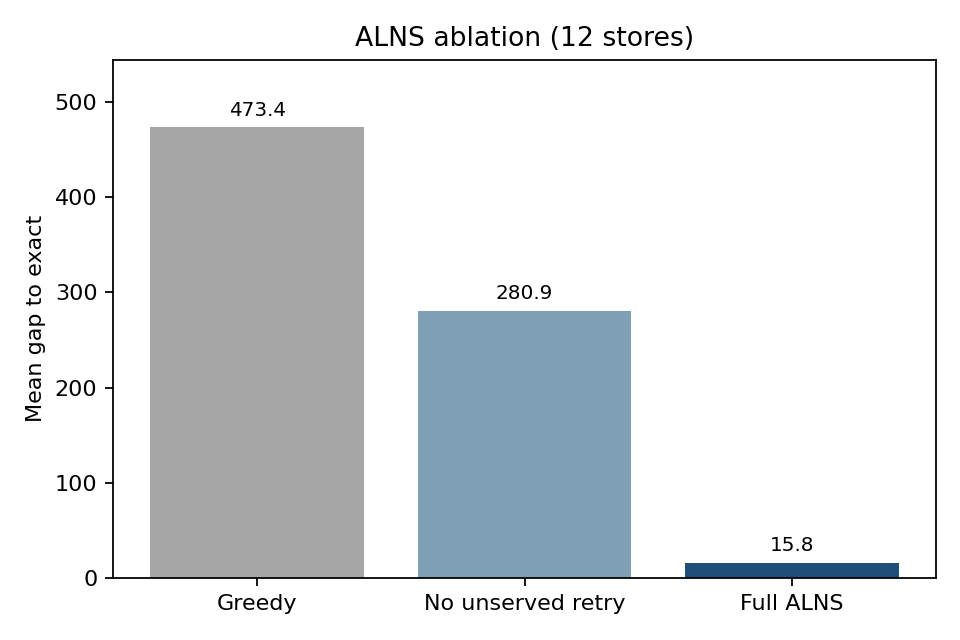
\includegraphics[width=0.72\linewidth]{figures/ablation.png}
\caption{ALNS ablation at 12 stores: mean gap to the exact optimum for greedy, no-unserved-retry, and full ALNS.}
\label{fig:ablation}
\end{figure}

\subsection{Practical policies and larger instances}

The three policies are evaluated against the exact optimum at 8 and 12 stores. At 8 stores, the mean gaps are 194.7 for nearest feasible, 36.2 for freshest feasible and 305.8 for oldest feasible; at 12 stores they are 259.9, 110.7 and 444.6. The freshest-feasible rule is the best simple policy and reaches the optimum in 4 of 10 eight-store instances and 2 of 10 twelve-store instances.

A stronger baseline adds 2-opt and relocate moves to the freshest-feasible solution, using the same age-feasibility check. At 8 stores it reaches a mean gap of 7.30 with 7/10 optima, so a rule plus local search nearly solves the small instances; the 95\% interval is $[-7.42,22.02]$, which includes zero. At 12 stores it reaches 67.10 with 2/10 optima and interval $[22.93,111.28]$, which excludes zero, while the held-out ALNS reaches 1.78 with 9/10. The comparison is therefore against an informed rule with local improvement, not only against an age-blind plan or a myopic rule, and the ALNS advantage survives at 12 stores.

\subsection{Mechanism and network design}

The $2\times2$ check separates the two components. With both age and MLOR removed, the age-aware and age-blind plans coincide, so the cold-chain label alone produces no decision difference. With MLOR only (all warehouses fresh), the mean difference is 74.0; with age only (all thresholds zero), it is 581.6; with both, it is 1003.6, larger than the sum of the parts. The interaction---matching inventory age to distance and store threshold---is the mechanism, not either component alone.

The difference is also visible in network design. At 8 stores, the age-aware plan opens the fresh warehouse in 10 of 10 instances, while the blind plan opens an old warehouse in 7 of 10; the open sets differ in 7 of 10 and the store-to-warehouse assignments differ in 7 of 10. At 12 stores, the open sets differ in 6 of 10, and the age-aware plan opens the fresh warehouse in 10 of 10 versus 4 of 10 for the blind plan. This is the decision consequence that makes the problem more than a routing constraint, although the three-warehouse design (one fresh, two old) makes the result less surprising than it would be with a richer age distribution.

\subsection{Sensitivity and lower bound}

The rejection penalty is varied from 0 to 800. At penalty 0, the age-blind plan is cheaper by 36.4 because it avoids the extra transport; from penalty 50 onward, the age-aware plan is better in all five instances (223.6 at 50, 483.6 at 100, 1003.6 at 200). With about 5.2 infeasible deliveries per instance, the break-even penalty is about 7 per delivery. The break-even is a model quantity, not an observed markdown cost.

\begin{figure}[t]
\centering
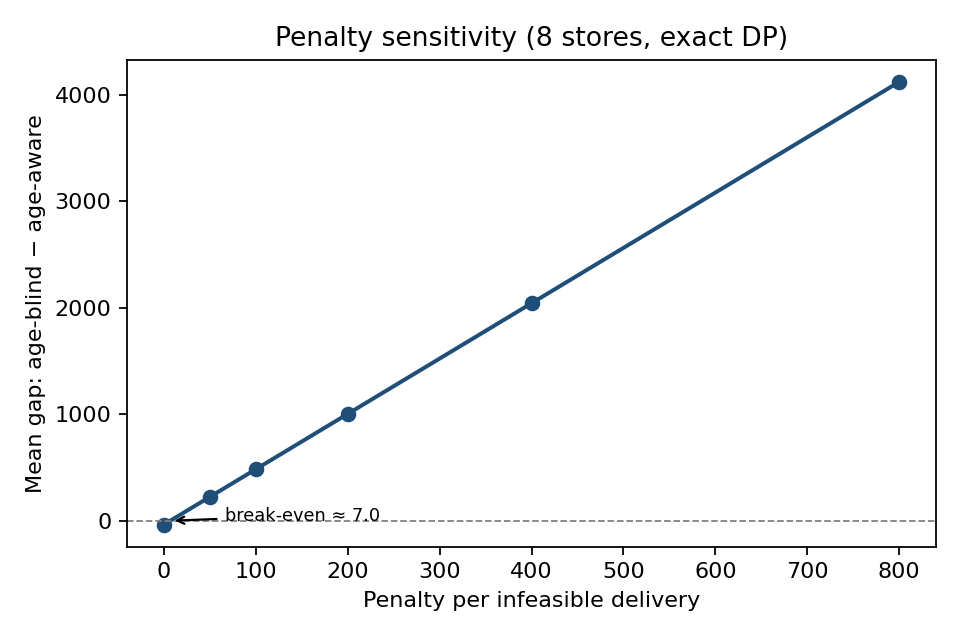
\includegraphics[width=0.72\linewidth]{figures/penalty.png}
\caption{Penalty sensitivity: mean gap between the age-blind and age-aware plans as the per-delivery rejection penalty grows; the break-even is about 7.}
\label{fig:penalty}
\end{figure}

At 20 stores, an LP relaxation of the set-partitioning model provides a lower bound. The LP allows fractional routes and fractional opening; the mean relative gap between the ALNS cost and this bound is 9.0\%, with a maximum of 14.1\%. Because the relaxation is weak, this is a loose upper bound on the true gap, not an optimality proof.

\subsection{Real-network illustration}

On the real-network instance, the greedy age-aware plan costs 2601.5, the blind plan costs 4884.9, and the ALNS reaches 2190.9, an improvement of 410.6 over greedy. The illustration shows that the mechanism survives on real geography and contest cost rates. It does not show that the model applies to real demand: the instance uses unit demand and rule-based ages and thresholds.

\subsection{What the experiments do and do not show}

The experiments support three claims: the age-aware plan is never worse than the age-blind plan on the tested instances; the ALNS is close to the exact optimum at 12 stores and improves greedy at 20 stores; and the age--distance--threshold interaction, rather than the cold-chain label, drives the difference. They do not support claims about optimality at 20 stores, about real demand, about multi-period inventory dynamics, or about a confirmed literature gap. Two qualifications follow from the intervals. The exact age-aware advantage is clearly positive at 8 and 12 stores (95\% intervals $[577,1526]$ and $[417,1819]$). The held-out ALNS gap and the tuning improvement are not statistically significant with ten instances; they are numerical, not proven.

\begin{table}[t]
\centering
\caption{Means and 95\% confidence intervals for the main comparisons.}
\label{tab:ci}
\begin{tabular}{lrr}
\toprule
Comparison & Mean & 95\% interval \\
\midrule
Exact age-aware advantage, 8 stores & 1051.3 & $[576.96,1525.64]$ \\
Exact age-aware advantage, 12 stores & 1117.8 & $[416.98,1818.56]$ \\
Held-out ALNS gap, destroy 4--6 & 1.78 & $[-2.25,5.81]$ \\
Held-out default gap & 13.43 & $[-12.78,39.63]$ \\
Paired difference, default minus tuned & 11.65 & $[-14.70,37.99]$ \\
Rule plus local search, 8 stores & 7.30 & $[-7.42,22.02]$ \\
Rule plus local search, 12 stores & 67.10 & $[22.93,111.28]$ \\
\bottomrule
\end{tabular}
\end{table}

Table~\ref{tab:runtime} reports single-process wall-clock time for three seeds per size. The exact DP is already slower than every heuristic at 12 stores (5.96 s versus at most 0.19 s), and it is not run at 20 stores. The four heuristics remain below 0.3 s at 20 stores. The ranking of heuristic times is not the ranking of solution quality: SA and tabu are faster than the ALNS but produce worse plans (Table~\ref{tab:meta}). Times are implementation- and machine-dependent and are not a hardware-independent benchmark.

\begin{table}[t]
\centering
\caption{Wall-clock runtime (seconds, mean over three seeds).}
\label{tab:runtime}
\begin{tabular}{lrrrrr}
\toprule
Stores & DP & ALNS & SA & Tabu & GA \\
\midrule
8 & 0.06 & 0.08 & 0.04 & 0.03 & 0.16 \\
12 & 5.96 & 0.10 & 0.04 & 0.02 & 0.19 \\
20 & -- & 0.18 & 0.06 & 0.01 & 0.26 \\
\bottomrule
\end{tabular}
\end{table}

\subsection{Managerial implications}

Four implications follow, conditional on the model and the synthetic instances. First, ignoring age is not only a routing error: it can change which warehouse is opened and which store is assigned, and the error appears at delivery as a rejected or downgraded load. Second, a freshest-first rule is a reasonable default for a planner who cannot optimize: it is the best of the three simple policies, while oldest-first (a FEFO-like rule) is the worst. Third, optimization pays mainly at 12 stores or more; at 8 stores a freshest-first rule with 2-opt and relocate is already close to the exact optimum, so the case for a sophisticated method is scale-dependent. Fourth, the break-even rejection penalty is about 7 per delivery in the synthetic scale: below it, the extra transport of age-aware planning may not pay; above it, it does. These are model-based statements, not field recommendations.

\section{Conclusions}

We studied a location-routing problem in which warehouse inventory age and a store-specific minimum remaining shelf life determine whether a delivery is acceptable. The shelf-life condition is an arrival deadline that depends on the serving warehouse's age; as a result, old inventory has a shorter effective service radius, and the assignment of stores to warehouses cannot be separated from route time. The exact subset dynamic program solves 8- and 12-store instances, and the age-feasible ALNS reaches the exact optimum in 9 of 10 held-out twelve-store instances with a destroy size selected on a development set. The mechanism check shows that the effect disappears when both age and MLOR are removed and is superadditive when both are present.

The results are conditional. The model is single-period, deterministic, single-echelon and unit-demand; stores have no inventory state, and the rejection penalty is a model device rather than an observed cost. A demand-weighted trial with contest demands (50--100 tons per day) degenerated because one visit per store cannot carry a city's demand, and it was reverted. Extending the model to split deliveries, multiple trips, store inventory, a second echelon, or multiple periods would change both the formulation and the solution methods.

The literature position is also conditional. The MLOR concept has been studied in an operations--marketing setting, and perishable inventory-routing models already track remaining shelf life; the closest location-routing work does not include a store delivery threshold, but the full text of one integrated production--distribution paper could not be obtained. Until that comparison is complete, the contribution should be read as a conditional decision mechanism, not as a confirmed new problem.

\appendix
\section{Evidence map}

\begin{table}[t]
\centering
\caption{Claim-to-experiment map.}
\label{tab:evidence}
\small
\begin{tabular}{p{4.6cm}p{7.0cm}}
\toprule
Claim & Experiment \\
\midrule
Exact age-aware versus age-blind, 8/12 stores & \texttt{mlor-dp}, \texttt{mlor-dp12} \\
Held-out ALNS and tuning & \texttt{mlor-holdout2}, \texttt{mlor-dp12-ext}, \texttt{mlor-dp12-ext2} \\
Strong baseline: rule plus local search & \texttt{mlor-policy-ls} \\
$2\times2$ mechanism check & \texttt{mlor-mechanism} \\
Network-design difference & \texttt{mlor-network} \\
Penalty sensitivity & \texttt{mlor-sensitivity} \\
LP bound, 20 stores & \texttt{mlor-bound} \\
Sequencing counterexamples & \texttt{mlor-sequence} \\
Confidence intervals & \texttt{mlor-stats} \\
Real-network illustration & \texttt{mlor-case} \\
Four-store brute-force correctness & \texttt{test\_mlor\_bruteforce} \\
\bottomrule
\end{tabular}
\end{table}

{\small\sloppy Full experiment directory names carry a date suffix (for example, \texttt{mlor-dp-20261028}); the table lists task names.

All experiment outputs are under \texttt{results/experiments/}; the DP and ALNS implementations are in \texttt{src/analysis/mlor\_dp2.py}, \texttt{src/analysis/mlor\_dp12.py} and \texttt{src/analysis/mlor\_alns.py}.}

\section*{Declaration of competing interest}

The authors declare that they have no known competing financial interests or personal relationships that could have appeared to influence the work reported in this paper.

\section*{Data availability}

All synthetic instances are generated by the code described in this paper. The real-network illustration uses the contest location, warehouse and order files. No confidential or proprietary data were used. The experiment outputs are stored under \texttt{results/experiments/} in the project repository.

\begin{thebibliography}{99}

\bibitem[Coelho and Laporte(2014)]{coelho2014}
Coelho, L.C., Laporte, G., 2014. Optimal joint replenishment, delivery and inventory management policies for perishable products. Computers \& Operations Research 47, 42--52.

\bibitem[Crama et al.(2018)]{crama2018}
Crama, Y., Rezaei, M., Savelsbergh, M., Van Woensel, T., 2018. Stochastic inventory routing for perishable products. Transportation Science 52 (3), 526--546.

\bibitem[Govindan et al.(2014)]{govindan2014}
Govindan, K., Jafarian, A., Khodaverdi, R., Devika, K., 2014. Two-echelon multiple-vehicle location--routing problem with time windows for optimization of sustainable supply chain network of perishable food. International Journal of Production Economics 152, 9--28.

\bibitem[Qiu et al.(2019)]{qiu2019}
Qiu, Y., Qiao, J., Pardalos, P.M., 2019. Optimal production, replenishment, delivery, routing and inventory management policies for products with perishable inventory. Omega 82, 193--204.

\bibitem[Rohmer et al.(2019)]{rohmer2019}
Rohmer, S.U.K., Claassen, G.D.H., Laporte, G., 2019. A two-echelon inventory routing problem for perishable products. Computers \& Operations Research 107, 156--172.

\bibitem[Singh and Kuthambalayan(2022)]{singh2022}
Singh, N.K., Kuthambalayan, T.S., 2022. Integrating operations and marketing decisions to manage perishability risks with target minimum remaining shelf-life available to consumers. Computers \& Industrial Engineering 163, 107812.

\end{thebibliography}

\end{document}
